A fundamental property of the Fourier transform is that the width of a
signal in time domain and in frequency domain are inversely related to
one another. This relationship is known as
the \emph{\index{time-frequency uncertainty principle}{time-frequency
uncertainty principle}}:
\begin{equation}
  \boxed{
  \Delta \omega \Delta t = \gamma 
    } \,\,.
     \label{eq:uncertainty}
\end{equation}
Here $\gamma \in \mathbb{R}$ is a real-valued constant, which is
dependent on how the ``width'' of a signal is defined in the time and
frequency domain, $\Delta t$ is the width of the signal in
time domain, and $\Delta \omega$ is the width of the same signal in
frequency domain.

Time-frequency uncertainty is a general relationship that applies to
Fourier transform pairs. The units don't have to be time and frequency. One such uncertainty rule in quantum physics is
the \emph{\index{Heisenberg uncertainty principle}{Heisenberg
uncertainty principle}} which states that the width of the momentum
wave function is inversely proportional to the width of the position
wave function.

\begin{marginfigure}
\begin{center}
\begin{tikzpicture}
	\begin{axis}[
        width=4cm,
        height=4cm,
        domain=(-10):(10),
        samples=300,
        xlabel={$t$},
        ylabel={},
        ymax=1.4,
        ymin=0.0,
        axis y line=none,
        axis x line=center, 
%        axis y line=center, 
        yticklabels={,,,}, 
        xticklabels={,,,}
    ]
    \addplot[blue] {exp(-1.3*x*x)};
    %    \addplot[red] {exp(-0.08*x*x)};
    \node at (axis cs:0.0,1.2) [above]{$\Delta t$};
    \addplot [dimen,black] plot coordinates {(-1.2,1.2) (1.2,1.2)};

\end{axis}

  \coordinate (v1) at (3.0cm,1cm);
  \draw (v1) node[above] {$\xleftrightarrow{\mathcal{F}}$};

	\begin{axis}[
        width=4cm,
        xshift=3.0cm,
        height=4cm,
        domain=(-10):(10),
        samples=300,
        ymax=1.4,
        axis y line=none,        
        ymin=0.0,        
        xlabel={$\omega$},
        ylabel={},
        axis x line=center, 
%        axis y line=center, 
        xticklabels={,,,},
        yticklabels={,,,},        
    ]
    \addplot[blue] { exp(-0.08*x*x) };
    
    \node at (axis cs:0.0,1.2) [above]{$\Delta \omega$};
    \addplot [dimen,black] plot coordinates {(-4.5,1.2) (4.5,1.2)};

\end{axis}
\end{tikzpicture}


\begin{tikzpicture}
	\begin{axis}[
        width=4cm,
        height=4cm,
        domain=(-10):(10),
        samples=300,
        xlabel={$t$},
        ylabel={},
        ymax=1.4,
        ymin=0.0,
        axis y line=none,
        axis x line=center, 
%        axis y line=center, 
        yticklabels={,,,}, 
        xticklabels={,,,}
    ]
%    \addplot[blue] {exp(-1.3*x*x)};
    \addplot[blue] {exp(-0.08*x*x)};
    \node at (axis cs:0.0,1.2) [above]{$\Delta t$};
    \addplot [dimen,black] plot coordinates {(-4.5,1.2) (4.5,1.2)};    

\end{axis}

  \coordinate (v1) at (3.0cm,1cm);
  \draw (v1) node[above] {$\xleftrightarrow{\mathcal{F}}$};

	\begin{axis}[
        width=4cm,
        xshift=3.0cm,
        height=4cm,
        domain=(-10):(10),
        samples=300,
        ymax=1.4,
        axis y line=none,        
        ymin=0.0,        
        xlabel={$\omega$},
        ylabel={},
        axis x line=center, 
%        axis y line=center, 
        xticklabels={,,,},
        yticklabels={,,,},        
    ]
%    \addplot[blue] { exp(-0.08*x*x) };
    \addplot[blue] { exp(-1.3*x*x) };    
    
    \node at (axis cs:0.0,1.2) [above]{$\Delta \omega$};
    \addplot [dimen,black] plot coordinates {(-1.2,1.2) (1.2,1.2)};
 

\end{axis}
\end{tikzpicture}

\end{center}
\caption{Above: A narrow signal in time domain is a wide signal in frequency domain. 
Below: A wide signal in time domain is a narrow signal in frequency domain.}
\label{fig:example_uncertainty}
\end{marginfigure}

\section{Example: Gaussian signal}
Figure \ref{fig:example_uncertainty} shows a graphical representation
of what Equation \ref{eq:uncertainty} means using a Gaussian signal, which has the following Fourier transform pair:
\begin{equation}
x(t) = e^{-\alpha t^2} \xleftrightarrow{\mathcal{F}} \hat{x}(\omega) = \sqrt{\frac{\pi}{\alpha}} e^{-\frac{\omega^2}{4\alpha}} \,\,.
\end{equation}
If we define the width of a Gaussian to be $x(\Delta t)=x(0)e^{-1}$ in
time domain and $\hat{x}(\Delta \omega)=\hat{x}(0)e^{-1}$ in frequency
domain, we find that $\Delta t = \alpha^{-1/2}$ and $\Delta \omega
= 2\alpha^{1/2}$. In this case, our time-frequency uncertainty rule would be:
\begin{equation}
\Delta \omega \Delta t  = 2 \,\,.
\end{equation}
What this relation means in practice can be seen in
Figure \ref{fig:example_uncertainty}. A Gaussian signal that is narrow
in time domain is wide in frequency domain. Conversely, a signal that
is wide in time domain is narrow in frequency domain.


\section{Time scaling}

Recall the time scaling system from the chapter on Fourier transforms,
which adjusts the width of a signal using the constant $\alpha$:
\begin{equation}
y(t) = x(\alpha t) \,\,.
\end{equation}
The Fourier transform of a time scaled signal $\hat{y}(\omega)$ is
scaled inversely in frequency:
\begin{align}
\boxed{
y(t) = x(\alpha t) \xleftrightarrow{\mathcal{F}} \hat{y}(\omega) = \frac{1}{|\alpha|}\hat{x}\left(\frac{\omega}{\alpha}\right)
} \,\, _.
\end{align}
What does scaling in time mean?
\begin{itemize}
\item compressing a signal in time with $|\alpha|>1$ will stretch the signal in frequency.
\item stretching a signal in time with $|\alpha|<1$ will compress the signal in frequency. 
\end{itemize}

\begin{marginfigure}[-6cm]
  \begin{center}
    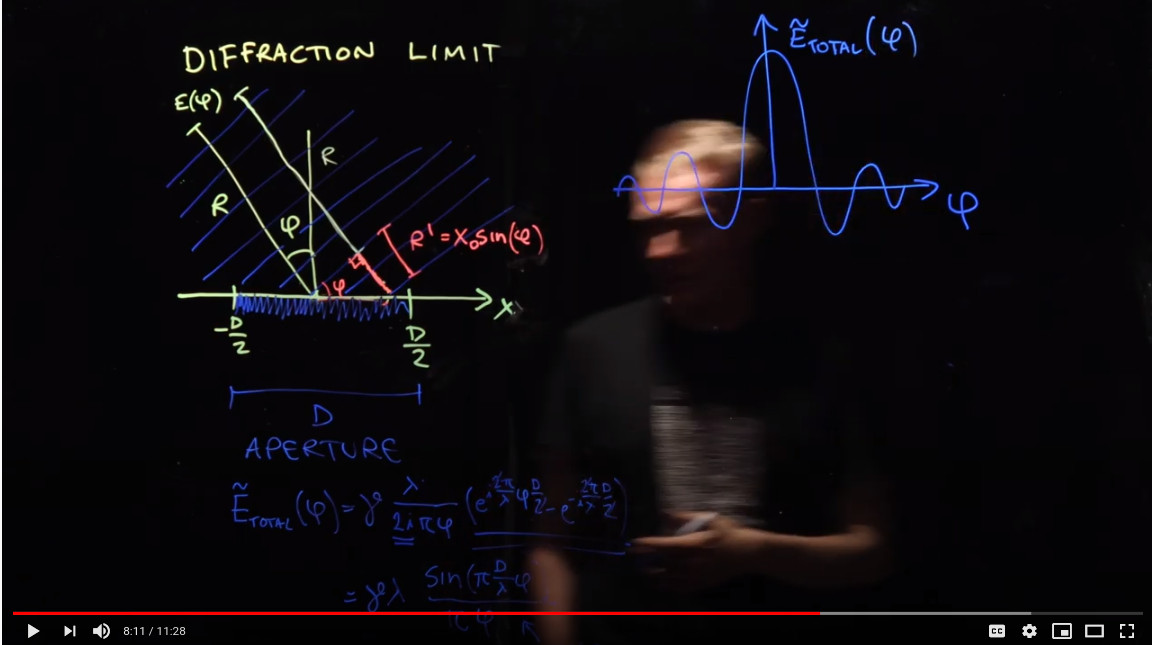
\includegraphics[width=\textwidth]{ch14/figures/video0.jpg}
  \end{center}
  \caption{A video deriving the diffraction limit from the Fourier transform relationship between an aperture diameter $D$ and the angular resolution $\Delta \phi$ \url{https://youtu.be/gKw46e4Ks4k}.}
\end{marginfigure}


\section{Example: Diffraction limit}


One example of the time-frequency uncertainty is the \emph{\index{diffraction limit}{diffraction limit}}
\begin{equation}
\Delta \varphi \Delta D=\lambda \,\,,
\end{equation}
which is encountered, e.g., in optics or in radio antenna theory. It
provides the theoretical limit for angular resolution $\Delta \varphi$
of an aperture with diameter $\Delta D$ that collects electromagnetic
waves. Here $\lambda$ is the wavelength of the electromagnetic waves
observed by the aperture. In this case, there is a Fourier transform
relationship between $\Delta \varphi$ and $\Delta D$. A derivation of
the diffraction limit using a basic Fourier transform pair was shown
in this video: \url{https://youtu.be/gKw46e4Ks4k}.



\begin{marginfigure}[-5cm]
\begin{center}
        \begin{tikzpicture}
        \begin{axis}[width=7cm,height=6cm,ymin=-0.5,xmin=-2.5,ymax=1.25,xmax=2.5,  yticklabels={,,},
        xtick={-2,-1,1,2},
         axis y line=none,
        xticklabels={$-\pi$,$-\hat{\omega}_0$,$\hat{\omega}_0$,$\pi$},
    xlabel=$\hat{\omega}$, axis lines = center]

\addplot[mark=none,color=blue] coordinates {
		(-2,0)
		(-1,0)
		(-1,1)
		(1,1)
        (1,0)
        (2,0)
	};

%\draw [gray, thick] (axis cs:-1,0.0) rectangle (axis cs:1,1.4);
   \node at (axis cs:0.7,1.05) [above, font={\footnotesize}]{$\mathcal{H}_{\mathrm{LP}}(\hat{\omega})$};


    \node at (axis cs:0.0,-.35) [above]{$\Delta \hat{\omega} = 2\hat{\omega}_0$};
    \addplot [dimen,black] plot coordinates {(-1,-.35) (1,-.35)};


\end{axis}
        \end{tikzpicture}
\end{center}
\caption{Ideal low-pass filter with cutoff $\hat{\omega}_0$ specified in discrete-time normalized angular frequency (radians per sample). 
The width of this filter in frequency domain is $\Delta \hat{\omega} = 2\hat{\omega}_0$.}
\label{fig:ideal_lpf}
\end{marginfigure}

\begin{marginfigure}
\begin{center}
        \begin{tikzpicture}
          \begin{axis}[domain=-7:7,
                       width=7cm,
                       ymax=0.7,
                       ymin=-0.4,
                       height=6cm,
                       xmax=9,
                       xmin=-9,
                       axis y line=none,       
                       xtick={-2,2},
                       xticklabels={$-n_0$,$n_0$},
                       yticklabels={,,},
                       xlabel=$n$, 
                       ylabel={$h[n]$},
                       axis lines = center]
            \addplot+[ycomb,opacity=0.3]{sin(0.5*3.14*deg(x))/(3.14*x) };

    \node at (axis cs:0.7,0.5) [above, font={\footnotesize}]{$h_{\mathrm{LP}}[n]$};
   
    \node at (axis cs:0.0,-.35) [above]{$\Delta n = 2 n_0 = 2\pi/\hat{\omega}_0$};
    \addplot [dimen,black] plot coordinates {(-2,-.35) (2,-.35)};

\end{axis}
        \end{tikzpicture}
\end{center}
\caption{The impulse response of an ideal discrete-time low-pass filter $h[n]$. The width of this filter in time domain is $\Delta n = 2\pi/\hat{\omega}_0$ (samples).}
\label{fig:lpf_impulse_resp_tf}
\end{marginfigure}

\section{Example: minimum length of a low-pass filter impulse response}

What is the minimum length required for a low-pass filter, in order to achieve a certain pass bandwidth?

Let's say that we wanted to low-pass filter a discrete-time signal
with a cutoff frequency $\hat{\omega}_0$. Figure \ref{fig:ideal_lpf}
shows the frequency response of an ideal low-pass filter. In this case,
$\Delta \hat{\omega} = 2\hat{\omega}_0$ is a measure of how wide the
filter is in frequency domain.

In the discrete-time Fourier transform chapter, we derived the impulse
response for the ideal low-pass filter to be:
\begin{equation}
h_{\mathrm{LP}}[n] = \frac{\sin(\hat{\omega}_0 n)}{\pi n} \,\, _.
\end{equation}
This impulse response is shown in
Figure \ref{fig:lpf_impulse_resp_tf}.

We'll define the time domain width using the approximate first zero
crossings of $h[n]$. This is denoted with $\pm n_0$ in
Figure \ref{fig:lpf_impulse_resp_tf}. We find that $n_0
= \pm \pi/\hat{\omega}_0$. Note that because this is a discrete-time
signal, there might not be an actual sample that is zero valued and
the value $n_0$ is the interpolated value where the impulse
response crosses zero. The total effective width of the filter in time
domain is then $\Delta n = 2\pi/\hat{\omega}_0$.

Now that we know the width in time and frequency domain, we can obtain
the product:
\begin{equation}
\Delta\hat{\omega}\Delta n = 4\pi \,\,.
\end{equation}
This is the time-frequency uncertainty principle applied to filter
design. This tells us that in order to make a low pass filter with
bandwidth $\Delta \hat{\omega}$, the impulse response of the filter
(the length of the FIR filter) needs to be at least $\Delta n \ge
4\pi/\Delta \hat{\omega}$ samples long.

Note that the value of this constant depends on the definition of the
width of the filter in time and frequency domain, and isn't
necessarily exactly $4\pi$. The only way to exhaustively characterize
the time and frequency domain properties of a signal is to investigate
the signal in time and frequency domain.

%Similar considerations apply to band pass filters, band-stop filters,
%and high-pass filters.

%Filters with sharp features in the frequency
%response of a filter can only be obtained with filters that have a
%long impulse response.

\if 0

\section{Example: Heisenberg uncertainty principle}

In quantum physics, the \emph{\index{Heisenberg uncertainty
principle}{Heisenberg uncertainty principle}} arises from the Fourier
transform relationship of momentum and position for a wave-packet that
describes a particle\footnote{Deriving this is outside the scope of
this course.}. It is defined as follows:
\begin{equation}
  \Delta x \Delta p \ge \frac{h}{4\pi} \,\, _,
  \label{eq:pos_mom}
\end{equation}
where $\Delta x$ is uncertainty in position, $\Delta p$ is uncertainty
in momentum $p$, and $h$ is the Planck's constant.

Using the Planck-Einstein relationship for photons moving at the speed
of light $c$, momentum is related to frequency as follows: $p=hf/c$,
where $f$ is frequency (cycles per second). Therefore:
\begin{equation}
  \Delta x \Delta f \ge \frac{c}{4\pi} \,\, _.
\end{equation}
In this case, the relation is between position uncertainty and
frequency uncertainty. 

\fi
